\section{Process' Perspective}

\subsection{Collaborative Development \& Team Organization}

When we initially talked about teaming up we made sure to align our expectations. We agreed that each member expected to spend 8-12 hours a week on the course. Thus our way of working became something like this:
\begin{itemize}
    \item Tuesday, 10-14: Project Work
    \item Tuesday, 14-16: Lecture
    \item Tuesday, 16-18: Exercises/Project Work
    \item Friday, 10-15: Project Work (When possible, not each Friday)
\end{itemize}

The above points were all physically present sessions for all members. Each member had the freedom to do additional work at other times during the week. All communication was through a Discord channel.

When working, we would at times do versions of pair programming. Teamwork was however difficult, since all concepts were new to everybody, and a lot of the understanding and progress came from trial and error. All sessions were an open forum where questions were welcome, and help was always possible to get. Sadly, we were not always good at remembering co-authorship on commits which might make the repository contributions look rather skewed.

We intended to utilize GitHub Issues to share the tasks between us, making sure not to be wasting time on duplicate work.


\subsection{CI/CD Chain}
%A complete description of stages and tools included in the CI/CD chains.
%That is, including deployment and release of your systems.
%- Github Workflows
%- Digital Ocean
% illustration af pipeline
% deployment and release
% hvilke ting kører vi hvornår og hvorfor


% Intro
In this project, we have implemented a CI/CD chain by defining a handful of \texttt{.yml} files that utilize GitHub Actions. 

Throughout the development stage of our chain, every time we pushed to a feature branch (more on branch strategy in section 2.3), the Super-linter is run except for pushes to main. This isbecause we primarily interact with main through pull-requests. During the development and refactoring of workflows, however, we did permit direct pushes to the main branch. The reason behind this was twofold: firstly, setting up secrets and forking the repository proved to be excessively time-consuming, and secondly, a failed workflow would not disrupt the functionality of our main branch. 
We also had a daily workflow using Dependabot, that scanned for outdated dependencies and informed us of updates through pull requests. Before any pull requests were merged into main, another developer had to perform a code review as part of our workflow. 

The first thing that happens when a pull request is created is that the application is built. Only building when a pull request is made to the main branch ensures multiple things:

\begin{itemize}
    \item Changes are isolated
    \item Since code is reviewed before a pull request is merged into main, code that is not reviewed is never deployed
    \item Overhead is reduced, by not running unnecessary build cycles on each push to a feature branch
\end{itemize}

As part of our build stage, we incorporate an additional formatter/linter that operates on the build. This step is implemented to guarantee a greater level of code consistency. Our build workflow proceeds by checking out the branch, restoring the dependencies, building the application and executing the unit tests. This makes the test-stage dependant on the build-stage; if the build fails, the tests are never run. Depending on the test-suite, stability is ensured by making sure changes are tested, and old functionalities do not break (regression testing).

As part of our testing we also implemented a Snyks workflow. Snyks is a security platform designed for finding vulnerabilities in open-source dependencies and doing security scans on the repository. Snyks is a great tool for notifying developers of any found critical vulnerabilities, that would pose a high threat to our application. Additionally, we used a Snyk feature on our code base, that scans the code base for sensitive data like connection strings, secret tokens, API keys, etc. This measure was taken in an effort to mitigate the risk of inadvertently exposing secrets.

\begin{figure}
    \centering
    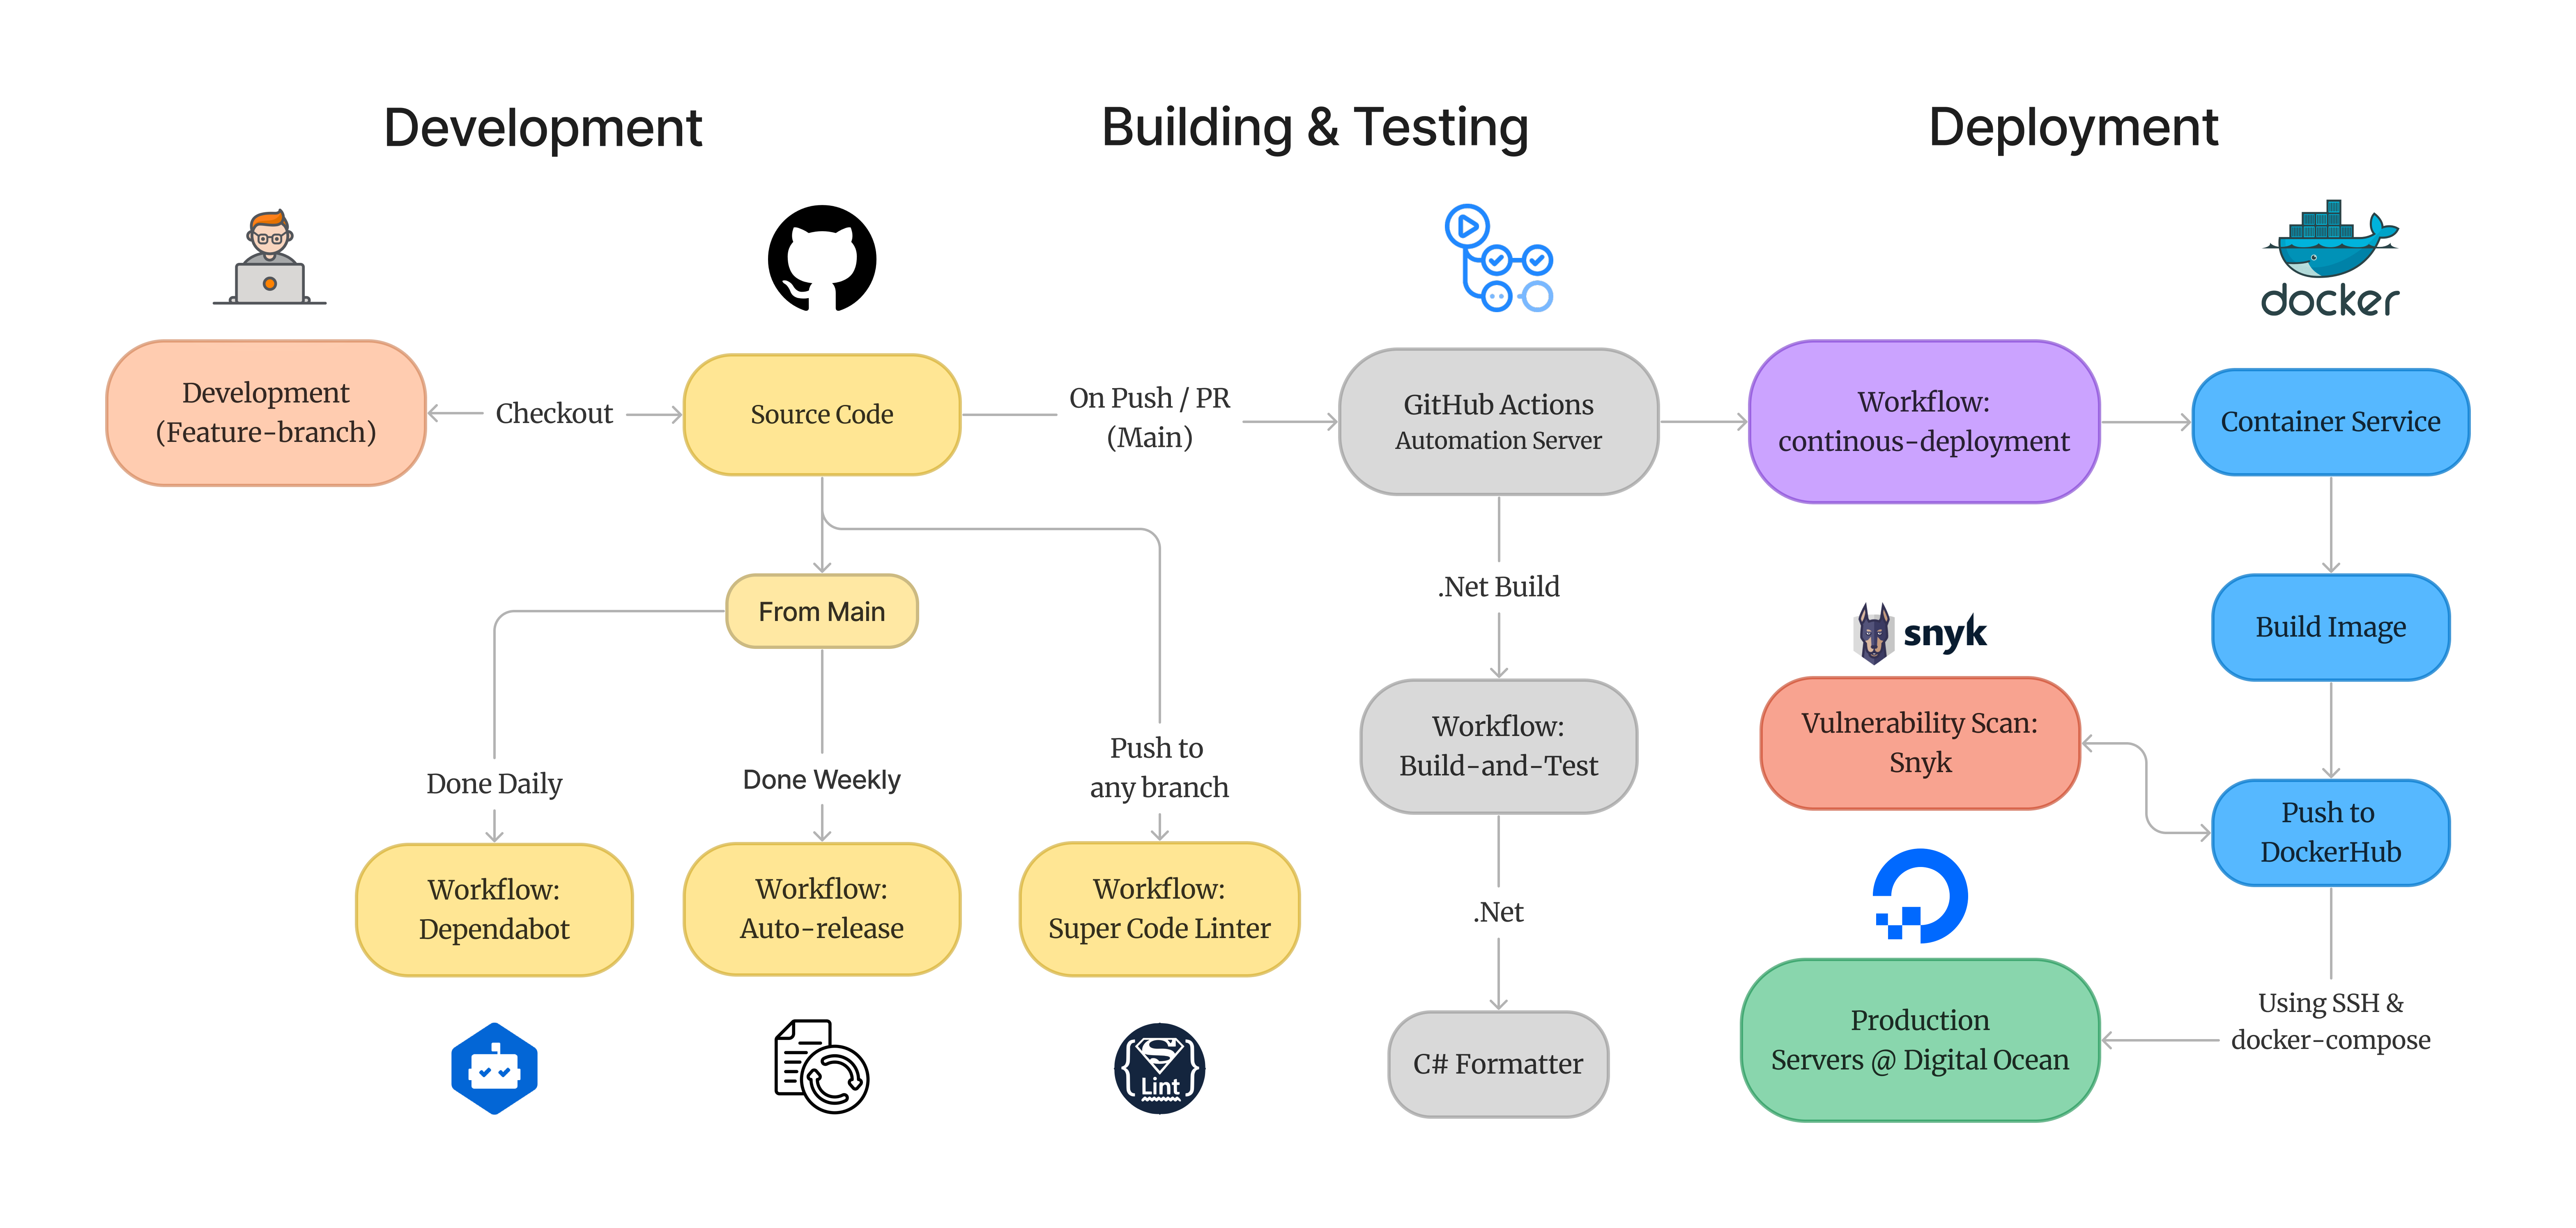
\includegraphics[width=1.0\linewidth]{Images/CICD_Chain.png}
    \caption{CI/CD tech-stack}
    \label{fig:CI/CD Overview}
\end{figure}

% Deployment workflow in detail:
After the build-and-test stage of the chain is run successfully, we move to the deployment stage. If either the building or testing fails, the pull request will be rejected.

We made a workflow, responsible for the continuous deployment aspect of the pipeline. Through this workflow, we have linked the building, testing, and deployment stages. Combined with the use of GitHub secrets, these workflows provide a powerful solution to automated deployment. Furthermore, it's a convenient way to manage our application's deployment process while maintaining confidentiality and flexibility. 
However, it does come with a drawback: Scalability is somewhat limited. One example of this is because the workflow uses repository secrets to reference the IP-addresses of our servers.
If we had been a 'real' company that wanted to change our Server-provider to something other than Digital Ocean, or perhaps just looking to add more servers, we would have to add a separate paragraph to the workflow and update the repository secrets \textit{manually}.

% (Release) workflow
\noindent As an additional last step, we implemented an auto-release function to further streamline the deployment process. This step ensured that the latest changes were automatically released as requested by TA's and teachers. This was a scheduled event, done each Sunday at 20:00 CEST. Another workflow that has to do with automating release, is the Latex workflow. This pulls the current version of the report, each time a push to main is made.

\subsection{Repository Organization \& Development Strategy}
\subsubsection{Repository Organization}

We structured our code in a mono-repository for two main reasons:
\begin{enumerate}
    \item It provides improved collaboration, as all developers are working on the same codebase.
    \item It simplifies version control as we only have a single history for all code.
\end{enumerate}
Another consideration was, that we didn't feel the need to divide it up, as the application is still relatively small. It would also add what we deemed to be unnecessary complexity by requiring different repositories to be cloud-hosted for cross-access since the necessary references in our C\# code would no longer reside in the same .NET solution.


\subsubsection{Development Strategy}

We utilized feature branching as our strategy as it has multiple advantages that work very well with the DevOps way of working. An example of this is continuous integration. The GitHub Actions make it simple to automate a require-to-pass test suite before any feature branch is merged into the main one. Other advantages include:

\begin{itemize}
    \item It isolates changes to specific features, minimizing conflicts with separate work.
    \item It facilitates the code review process that in turn ensures quality assurance.
    \item It provides a clear separation of work, which makes collaboration easier.
    \item It makes parallel development possible.
\end{itemize}

Our tasks were organized in GitHub Issues. This made it possible for each member to always be able to see which tasks were up for grabs, and who were working on what. It also acted as a task backlog giving an overview of the work that was yet to be done.

\noindent As the project progressed, however, the tasks began including the whole group, and the Issues board became slightly irrelevant.

\subsection{Monitoring \& Logging}
%How do you monitor your systems and what precisely do %you monitor?
%What do you log in your systems and how do you %aggregate logs?

\subsubsection{Monitoring} \label{Monitoring}

We monitor our system by having Prometheus gather metrics from our metric endpoints regularly. This is made possible by the NuGet package Prometheus.net, which is responsible for exposing a metrics endpoint in our API, which Prometheus can then send requests to. This data is then queried again by Grafana, which is responsible for visualizing it. We can access Grafana's dashboard through the user we set up. Our current metrics are:

\begin{itemize}
    \item Http-requests (Duration)
    \item Total Users
    \item Total Messages
    \item Average request duration (Last 2 minutes)
\end{itemize}

\noindent Together, these metrics provide information about how much stress we can expect our system to experience, and what kind of request intensity we can expect. It also provides an overview of user growth, giving us a sense of the direction our service is headed. 

Additionally, we are also making use of Digital Ocean to monitor our hardware such as the CPU and memory usage of our droplets.

\subsubsection{Logging} \label{Logging}

To implement logging in our project, we used Serilog to do the actual logging, elastic search as the database to hold the logs and Kabana which serves as a UI to view them.
In order to log we are making use of the Serilog.Sinks.Elasticsearch NuGet Package. In our application, we have specified some metrics that ElasticSearch 

Kibana then retrieves the logging data from this sink and displays it.
We are logging all exceptions, requests to the controllers, and different functionalities happening in the middleware. 

skiftet default logger ud med serilog - andet format 
alle logs vi får er logs fra middleware 
default configuration logs - 


Log messages are generated to capture important events, errors, or relevant information during runtime. These logs are collected and forwarded to ElasticSearch, that then indexes and stores the data. Kibana then connects to ElasticSearch 

we use - sink direkte fra .NET direkte ind til (serilog - logging framework). en sink, der hvor alle logs glider hen. Den sink er sat til elastik search hvor kibana kan vise os logs på en pæn måde.
sender det videre til elastisearch direkte
det er kun logs fra .Net så vi kan formattere det her og fortælle hvad vi gerne vil logge og hvordan det skal se ud direkte i serilog. 
der er formartering i serverens programfil, men bliver måske ikke brugt ved deployment. 
triggers i middleware. når vi modtager request bliver der lavet en log, når den er færdig med at processe - værktøjer der laver logs for os. 

alle exceptions
request til controllers
masse andre ting der er I middleware - 


\subsection{Security Assessment}

Our security assessment consisted of a penetration test - Zed Attack Proxy, or ZAP, that showed some flaws in our program. Most seemed to be relatively simple to fix, and none seemed to be too severe in nature:
\begin{itemize}
    \item No Anti-CSRF tokens were found in a HTML submission form
    \item Passive (90022 - Application Error Disclosure)
    \item Content Security Policy (CSP) Header Not Set
    \item Missing Anti-clickjacking Header
    \item X-Content-Type-Options Header Missing
    \item Hidden File Found
    \item Vulnerable JS Library
    \item XSLT Injection might be possible.
    \item Cloud Metadata Potentially Exposed
\end{itemize}

\noindent These items resulted in GitHub Issues; some of which were dealt with while others were down-prioritized.

\subsection{Scaling \& Load Balancing}
%Applied strategy for scaling and load balancing. 

Our applied strategy for scaling and load balancing involved utilizing Docker Swarm for fault tolerance and easy container management, together with Nginx working primarily as a load balancer and reverse proxy. Docker Swarm uses a cluster of nodes (workers and managers) and allows us to automatically adjust the number of running Docker containers based on the current workload. Another important feature of the swarm is that it automatically evenly distributes incoming requests across the worker containers running the same service (internal load balancing with an ingress mesh).

The swarm has a maximum capacity limited to the combined resources (CPU, memory, disk space) of the server nodes within the swarm clusters. We used two servers for our application swarm and one server for the load balancing swarm.

The first swarm consists of a server with manager nodes, and a server with worker nodes running containers with our MiniTwit application. The second swarm includes a single manager node responsible for load balancing and reverse-proxying with Nginx. We designed it this way to separate concerns and allow the two swarms to scale independently. Combining Docker Swarm's automatic and dynamic scaling with Nginx's reverse-proxy capabilities resulted in an improvement in the system's availability and reliability.

By having Nginx handle and redirect request to our service, we could eleminate the 'single point of failure', and decrease the impact a server-crash has on our system. In case the primary replica-node running our swarm was flooded or broke down, we could redirect the trafic from that server-node to another upstream server, while docker swarms dynamical scaling would ensure that the system would be able to keep up with accelerating request and users.

However, in our setup, there were a couple of things that could be improved.
Initially, we only tested our system using a single instance of Nginx, which essentially only shifted the singel point of failure from the application service to the load-balancer in the Swarm. This decision involved weighing the trade-offs between reliability, complexity and also the financial costs of creating more droplets.
Also, we encountered some non-negligible internal network delays that affected the system's performance. When Nginx was responsible for the load balanceing, request took a long time to complete or re-direct. Due to the way Nginx was implemented it didn't function as originally intended.


%------ Asger 21-05-23 ------
% Har læst det igennem forklarret om docker swarm intern load balanceing og Nginx som ekstern loadbalanceing og fault tolerance. Tilføjet lidt mere detalje om hvorfor vi har to swarms og hvordan vores setup er + begrundelser.
% Vidste ikke helt noget om dette:
% Det interne netværk skulle have tilladt redirection, men gjorde det ikke ?

% ----- noter fra før: ------
%loadbalancer: nginx, reverse proxy, delay
%- det var meningen at den skulle tage sig af redirection, men det virkede ikke som om at vi kunne det.

\subsection{AI Assistance}
%In case you have used AI assistants for writing code during your project or to write the report:
%Explain which system(s) you used during the project.
%Reflect on how it supported/hindered your process.
%In essence, it has to be clear how code or other artifacts come from ideas into the running system and everything that happens on the way.



As developers, we have embraced the tool that is AI. We have used ChatGPT as a sparring partner whenever we got a task we did not know how to solve, or when we got stuck. It has been mostly great at providing ideas or starting points, but it has probably been at its best when troubleshooting or debugging. If nothing else it has provided the services of a rubber duck.

We have also used it in the formulation of documents like the SLA agreement, as it is mostly boilerplate text anyways. We provided it with some information about our system and what guarantees we could give, and it returned a rough draft we could finalize.

Finally, one team member has been using GitHub Copilot as an advanced intellisense tool, but not for making several lines of code. Meaning that it was used to finish individual lines of code, but not for making entire methods or blocks of code.